\section{Strategy} \label{sec:Strategy}

In most searches for physical processes in particle physics data, a simulation template is formed and is then fit to data in a given signal region in order to determine if the expected physical process in present in the data. Typically the signal region is a single variable, or set of variables where more signal than background is expected. In this analysis, the signal region used to fit the simulation template to data is the diphoton invariant mass, in the window 115 $<$ $\mgg$ $<$ 135. This region is chosen due to the expectation that the H$\rightarrow\gamma\gamma$ leg of the HH$\rightarrow$WW$\gamma\gamma$ process should provide a peak in this region.

There are two background signatures present in this analysis: A resonant background from the single Higgs to $\gamma\gamma$ process, and a continuum background formed by a combination of background processes which do not contain a prompt diphoton. An illustration of the signal and background signatures is shown in Figure \ref{fig:Signatures}.

\begin{figure}[h!]
    \centering
    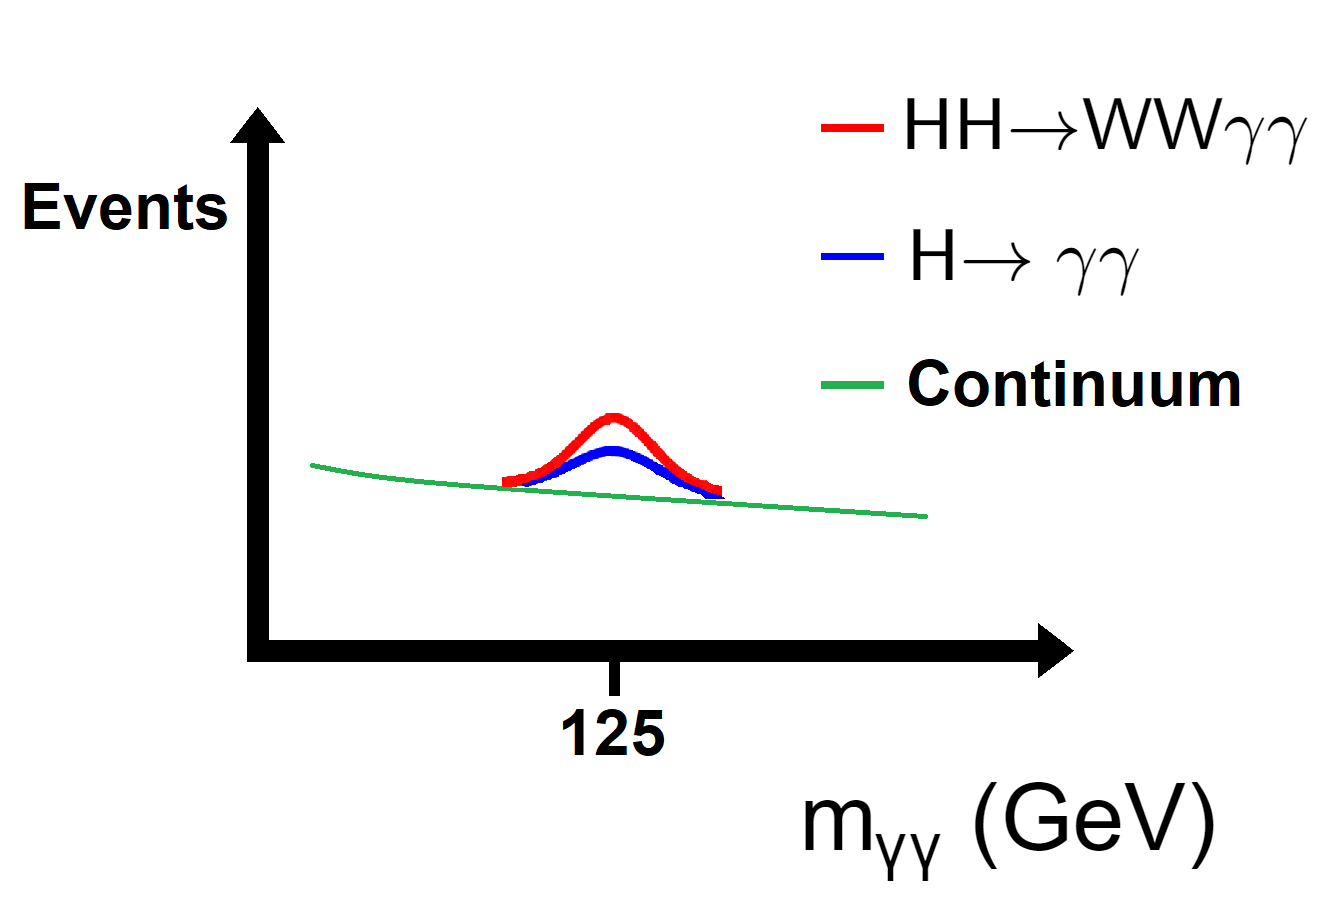
\includegraphics[width=0.75\textwidth]{Sections/HHWWgg/images/Strategy/HHWWgg_ResbkgPlot.png}
    \caption{Analysis signal and background signatures.}
    \label{fig:Signatures}
\end{figure}

In order to optimize the sensitivity of this analysis,
a DNN (Deep Neural Network) is employed for the Semi-Leptonic final state, as it is expected to be the most sensitive channel due to the increase in branching ratio
from the hadronic W decay, but with the benefit of maintaining a clean signature due to the presence of a lepton. A multiclass DNN is trained in order to separate the SM di-Higgs signal from background processes, while a binary parametric DNN is used to differentiate 20 EFT benchmark scenarios from background processes.

The FH channel also uses a DNN in order to optimize sensitivity, in this case by separating FH HH signal from backgrounds. In the FH channel, there is a significant overlap with the $HH\rightarrow$bb$\gamma\gamma$ final state, so two binary DNNs are trained:
The first binary DNN separates the FH WW$\gamma\gamma$ process from all backgrounds, and is used for categorization. To reduce the overlap of bb$\gamma\gamma$ events between the bb$\gamma\gamma$ and WW$\gamma\gamma$ phase spaces,
another binary DNN is trained that separates bb$\gamma\gamma$ from all backgrounds. The bb$\gamma\gamma$ training score is used as a ``bb$\gamma\gamma$ killer'', where a selection is applied on its value
to reduce the contamination of bb$\gamma\gamma$ events in the WW$\gamma\gamma$ phase space, while preserving the majority of WW$\gamma\gamma$ signal events. 

For the Fully-Leptonic channel, a cut based strategy is used due to a lack of number of events necessary to perform an MVA (Multivariate analysis) training. 

It is imperative to apply orthogonal selections to data and simulation events in order to avoid including the same events in multiple background categories. This is done via the event's number of leptons, where
each lepton must pass a common set of selections applied for all final state tags. After a set of lepton objects is selected for each data or simulation event, events fall into the FH category if they contain exactly zero leptons, the SL category if they contain exactly one lepton and the FL category if they contain exactly two leptons.

Further event selections are made for the three final state categories,
but by requiring an orthogonal separation of the number of leptons, it is guaranteed no one event can fall into more than one category. Thus, a simultaneous fit of background and signal models to data 
in different final state categories can be performed in order to obtain a final result which benefits from a combination of the physics signatures of all three final states. This is also summarised in the flow chart shown in Figure \ref{fig:HHflowChart}.

\begin{figure}[h!]
    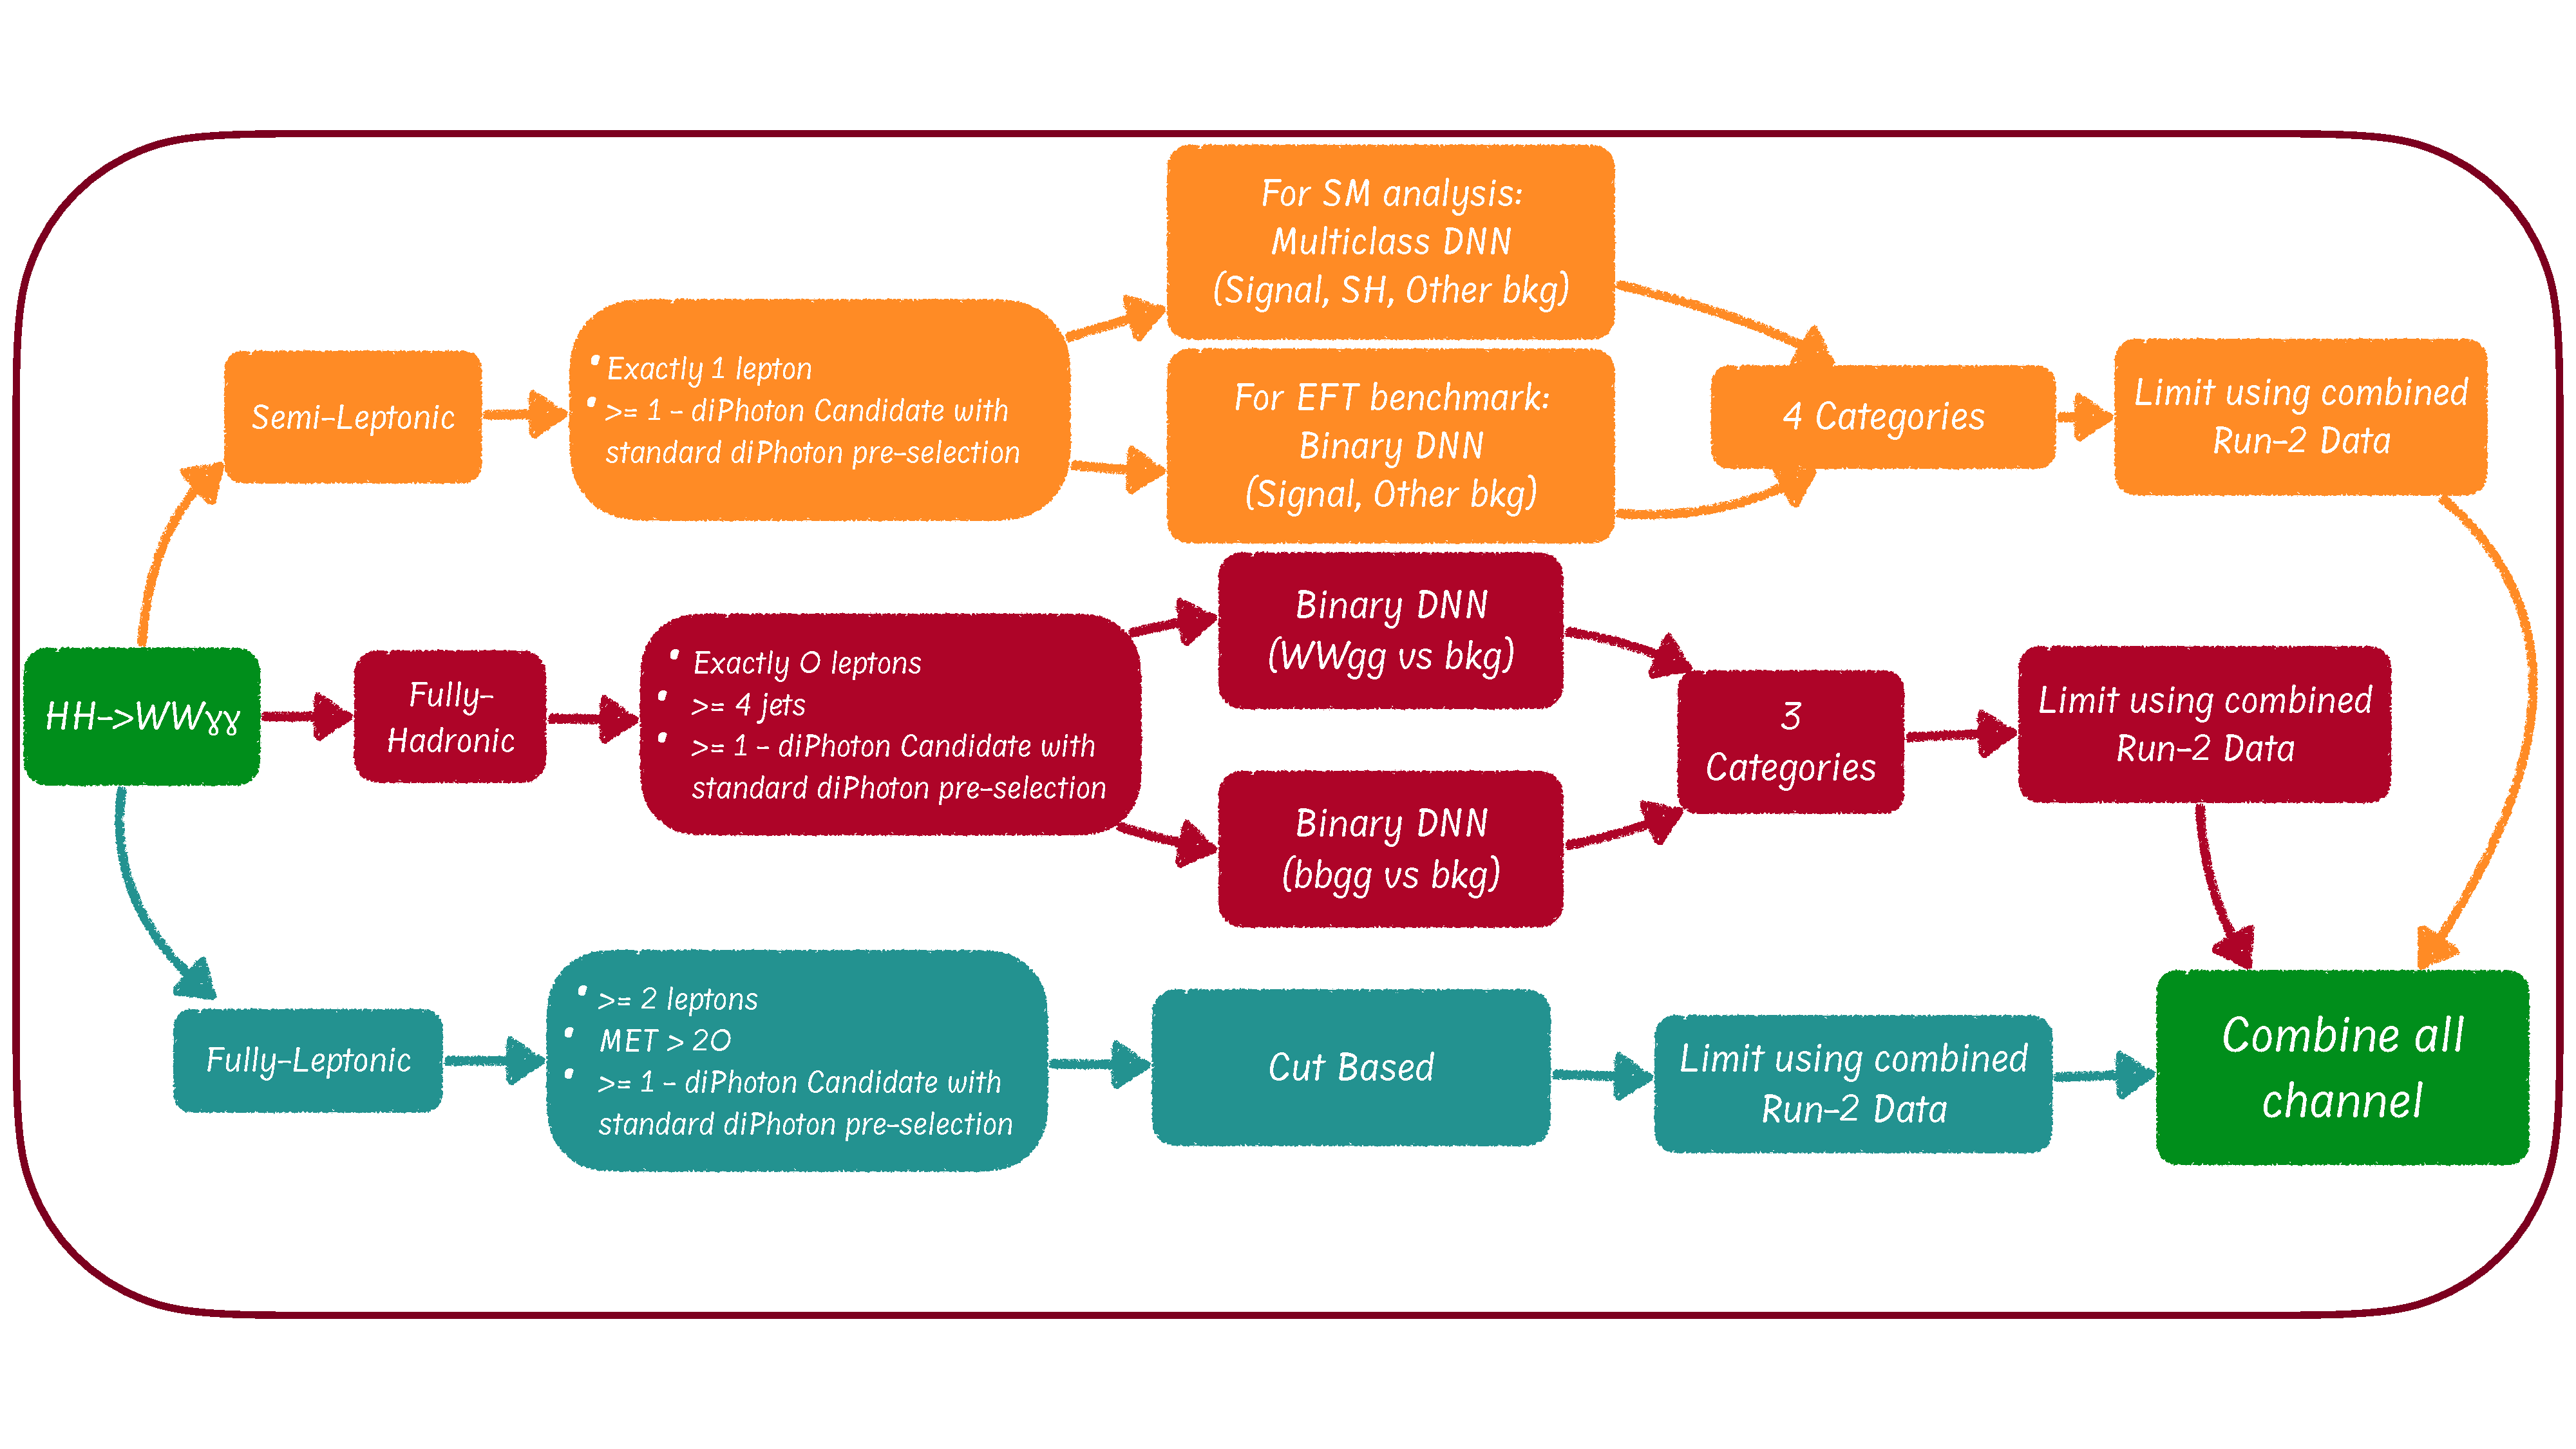
\includegraphics[width=\textwidth,trim={0 3cm 0 3cm},clip=true]{Sections/HHWWgg/images/Strategy/HH_flowchart.pdf}
    \caption{$HH\rightarrow WW\gamma\gamma$ Analysis flow chart}
    \label{fig:HHflowChart}
\end{figure}

Signal and background models are constructed independently for each year of data and MC (2016, 2017 and 2018) and combined to produce signal and background models to fit to the LHC Run 2 dataset. Results are obtained by performing a simultaneous
likelihood fit to the invariant diphoton distribution, \mgg, among all categories. This procedure is performed in order to extract 95\% CL upper limits on di-Higgs production within the context of the SM interpretation. Additionally, through the use of an EFT lagrangian, various simulation templates are fit to data and a linear combination of EFT samples results in the scan of two EFT parameters, and upper limits are extracted on 20 EFT benchmark scenarios. 